\documentclass[sigconf, nonacm=true]{acmart}


\settopmatter{printacmref=false}
\setcopyright{none}
\renewcommand\footnotetextcopyrightpermission[1]{}
\pagestyle{plain}
\hypersetup{
    colorlinks=true,
    linkcolor=blue,
    filecolor=magenta,
    urlcolor=cyan,
}

\usepackage{CJKutf8}
\usepackage{graphicx}
\graphicspath{./image/}

\defcitealias{semaphore}{Semaphore}

\title{Mitigating the Effects of COVID-19 via an Anonymous Authentication System and Zero-Knowledge Proofs}
\subtitle{CNS Term Project Proposal}
\author{
    R08922161 \and
    M10915072 \and
    B08902124 \and
    B05901044
}

\begin{document}

\maketitle

\section{Abstract}

COVID-19 has resulted in a significant number of fatalities worldwide, and has brought with it significant challenges that require coordination on an international level. Such coordination requires widespread knowledge of vaccination and quarantine information, but public availability of such knowledge could potentially leak user data and could have long-term privacy concerns. We propose researching state-of-the-art techniques for anonymous authentication systems, as well as implementing a proof-of-concept anonymous authentication system using Zero-Knowledge Proofs, which could be extended into a vaccine authentication system or quarantine assurance system with emphasis on maintaining the privacy of individuals.

\section{Motivation}

Mitigating the spread of sicknesses such as COVID-19 results in several challenges that must be addressed at a societal level, which requires both widespread coordination as well as assurances in the accuracy of available information. However, making certain information public and widely accessible can bring with it certain privacy concerns when such information involves personal medical data. We believe that for mitigating the effects of the pandemic, it is important for people to know who may be sick, who may have been exposed, and who should be in quarantine, but we also recognize that the widespread availability of user medical data could potentially have long term effects on the privacy of individuals, and we recognize that that is a valid concern. Our work seeks to address this challenge through the use of Zero-Knowledge Proofs (ZKP), with a particular focus on providing methods for vaccine verification and for ensuring people stay in quarantine, while simultaneously maintaining the privacy of individuals. In doing so we will attempt to create a proof-of-concept of an \textbf{Anonymous Authentication System} that could be applied to the challenges of containing COVID-19.

Zero-Knowledge Proofs refer to computational methods that can be used to assert whether or not a given piece of data is contained within a specific set of data, without actually revealing the data. Doing so typically involves generating a proof with a logic circuit that asserts that the given data is present in a set of data particular to the circuit, and afterward the proof can be presented to others and verified with the circuit in lieu of revealing the original data.

Fortunately, the implementation of ZKP has become significantly more practical with regard to general programming due to techniques developed by Gennaro et al. and other developer-friendly tools becoming available \cite{GGPR13}. Consequently, we propose to not only perform general research with regard to developments with ZKP technology as present in the literature, but also to attempt to implement such a system using modern tools. Our system should act as a proof-of-concept for a vaccine verification system or a system to ensure individuals stay in quarantine.

\section{Related Work}

\citetalias{semaphore} is an example of ZKP technology that allows users to prove their membership of a set without revealing their original identity on Ethereum. At the same time, it allows users to signal their endorsement of an arbitrary string. To our knowledge, ZKP technology has not been applied to mitigating the effects of the pandemic.

The pandemic has had a significant impact on tourism, the restaurant industry, and local businesses. Currently, countries are preparing to loosen restrictions to lessen the economic impact of the pandemic. Countries such as Iceland, Thailand, and Hong Kong have proposed policies that allow opening borders to people who can prove they have been vaccinated. Proposed authentication methods typically involve the presentation of a paper certificate, such as the Health Pass proposed by the European Union, and the IATA Travel Pass by Singapore Airlines. Mobile applications have also been used to obtain and verify personal medical information for this purpose.

\section{Plan}

To obtain a better understanding of the current state of research regarding anonymous
authentication systems, we will first perform a comprehensive literature survey on techniques and methods used to perform Zero-Knowledge Proofs. Doing so should give us a better understanding of current challenges faced with regard to anonymous authentication systems, as well as give as a better understanding of not only how to implement such a system, but on state-of-the-art methods and techniques that can be employed to achieve performance benefits and better privacy assurances.

Our first focus will be on understanding the implementation of the ZKP system by Groth et al. (\cite{Gro16}), which to our knowledge provides a state-of-the-art high level interface for an easier development of programmable Zero-Knowledge Proofs. The system uses \href{https://github.com/iden3/circom}{Circom}, which is a programming language specifically designed for the implementation of Zero-Knowledge Proof circuits.

Finally, we intend to implement an anonymous authentication system with a Zero-Knowledge Proof circuit
and then build a vaccine certificate and quarantine assurance system above it to show how it might help
in real world situations, particularly with regard to mitigating the current pandemic.

\section{Timeline}
We are going to have a checkpoint per week, and here is our goal to check in
each checkpoint:
\begin{enumerate}
    \item \textbf{05/11} - Having understanding about current solutions and
    problems about anonymous authenticate system.
    \item \textbf{05/18} - Having understanding about how \cite{Gro16} works and
    able to build general program in
    \href{https://github.com/iden3/circom}{Circom}.
    \item \textbf{05/25} - Finish the specification of the anonymous
    authentication system and vaccine certificate system we are going to build.
    \item \textbf{06/01} - Finish anonymous authentication system.
    \item \textbf{06/08} - Finish vaccine certificate system and quarantine assurance system and TUI client to interact with it.
\end{enumerate}

\section{Deliverables}
In the end of this term project, we expect to deliver:
\begin{itemize}
    \item A research report about anonymous authentication system implementations
    \item A proof-of-concept anonymous authentication system built with ZK-SNARK
\end{itemize}

Our proof-of-concept system would attempt to simulate how such an anonymous authentication system would be applied on a larger scale. As such, central authorities such as governments or hospitals, as well as end users, would all be simulated in our proof-of-concept system.

Our anonymous authentication system assumes a central authority could update a database containing a set of IDs unique to individuals in a certain population, for which the Zero-Knowledge Proof system could be used to prove whether or not a certain ID is contained within the set. The set in question could represent individuals currently in quarantine, or individuals who have become vaccinated. We plan to simulate this setup and behavior with generated IDs, to simulate how a central authority such as a government could utilize our system.

In the case of vaccine authentication, after a given user has been vaccinated, they could download a COVID-19 Vaccine Passport app and then register with the central authority. Alternatively, this could be done on behalf of the user by the hospital administering the vaccine. In the case of quarantine verification, this could be handled by the central authority (i.e., a government) directly.

\begin{figure}[H]
    \centering
    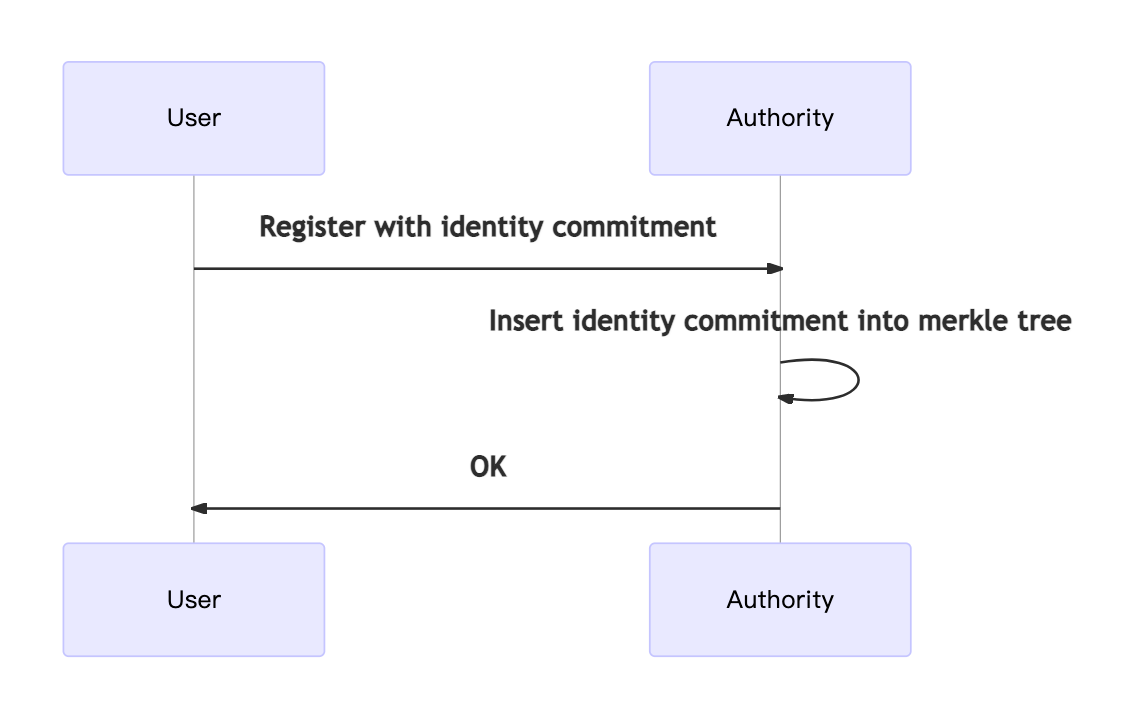
\includegraphics[width=6cm]{image/registration.png}
    \caption{Registration}
    \label{fig:reg}
\end{figure}

When a user would go someplace such as a store or movie theater, the place may wish to receive proof that the user has been vaccinated or is not supposed to be in quarantine. As such the user could provide a proof that does not reveal the user's identity.

\begin{figure}[H]
    \centering
    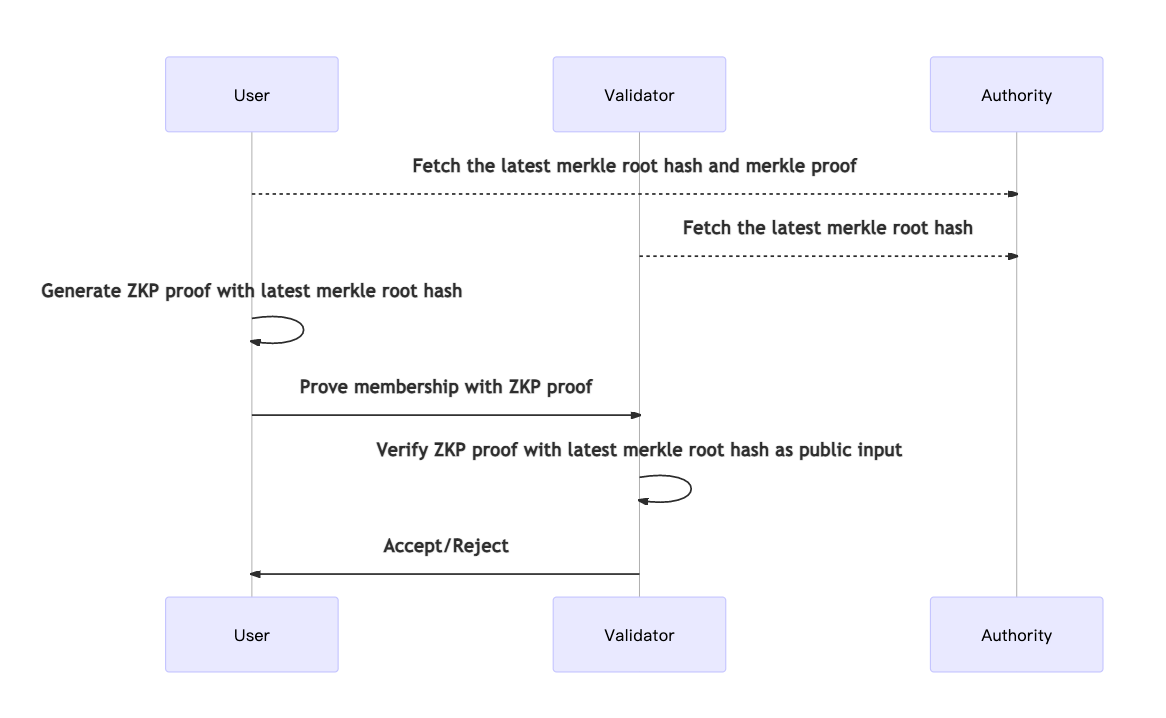
\includegraphics[width=6cm]{image/authentication.png}
    \caption{Authentication}
    \label{fig:auth}
\end{figure}

We assume the lifetime of a merkle tree would be for a selected amount of time, after which the tree would update from the set controlled by the central authority, and every user would automatically fetch the latest merkle root hash and merkle proof, and all validators would fetch the latest merkle root hash at consistent time intervals. As such, new user IDs could be added to the merkle tree upon vaccination, or upon being placed in quarantine. In the case of quarantine, user IDs could expire from the set after a set amount of time, representing the duration of the quarantine.

\begin{figure}[H]
    \centering
    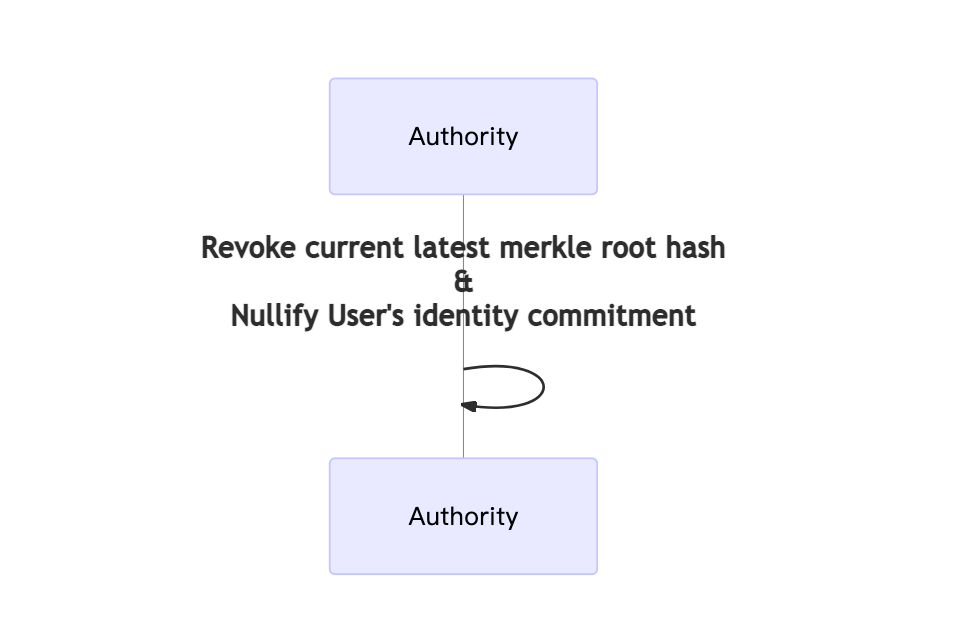
\includegraphics[width=6cm]{image/revocation.png}
    \caption{Revocation}
    \label{fig:rev}
\end{figure}

We also plan on assessing possible ways that end users could potentially abuse our system, in an effort to improve robustness, efficiency, and privacy of the system.

\bibliographystyle{alpha}
\bibliography{references}

\end{document}
